\documentclass{report}
\title{Susquehanna User Manual - v0.2.0 Cliffside}
\date{\today\\Revision 5}
\author{thetacola}
\usepackage{graphicx}
\usepackage{indentfirst}
\usepackage{wrapfig}
\usepackage{tcolorbox}
\usepackage{tipa}
\pagenumbering{arabic}

\begin{document}
	\tcbset{colback=purple!5!white,colframe=purple!75!black}
	\begin{figure}
		\centering
		\includegraphics[width=0.7\linewidth]{img/logo}
	\end{figure}
	\maketitle
	\tableofcontents
	\chapter{Introduction}
	\begin{figure}[ht]
		\centering
		\includegraphics[width=1\linewidth]{img/diagram}
		\caption{The three main components, labeled.}
		\label{fig:tabs-diagram-1}
	\end{figure}
	\par
	Susquehanna is a program made for the creation and management of conlangs. This application may also find use as a tool for the documentation of natural languages. Note the three main parts of the interface in Figure \ref{fig:tabs-diagram-1}, those being the tabs, the tools, and the book. The tabs categorize tools into groups, the tools allow the user to switch between books, and the book allows the user to interact with the language. The following sections will allow you to become familiar with these parts of the interface. As of this version, Susquehanna autosaves all changes as soon as they are made, so one does not have to worry about data loss.
	\section{Tabs}\label{sec:tabs}
	\begin{wrapfigure}{r}{0.5\textwidth}
		\centering
		\includegraphics[width=0.038\textwidth]{img/tabs-screenshot}
		\caption{The six tabs in Susquehanna.}
		\label{fig:tabs-screenshot}
	\end{wrapfigure}
	Tabs can be found on the leftmost edge of the application whenever it is open. These tabs categorize tools into categories,	so that each tool is easier to find. These tabs are also color coded, and the color of the book background is decided by the currently selected tab. To check which tab is being used, the user can see which color book background matches which color tab.
	\par
	There are six tabs, those being File, Phonology, Orthography, Grammar, Lexicon, and Settings. This manual covers each tab in detail, for more information on each tab please check the table of contents to find the page about a given tab. When using Susquehanna on low-resolution displays or small window sizes, the tabs can be scrolled through using the scroll wheel. Using the PgUp and PgDown keys on the number pad also works. 
	\par
	\begin{tcolorbox}[width=1\textwidth]
	\textsc{For developers:} Adding a new tab to Susquehanna is fairly simple. This can be done by editing \emph{net.oijon.susquehanna.gui.Navbox}. First, create an image for your new tab. A template for this can be found in \emph{src/main/resources/img}. Save your image as \emph{\{name\}-tab.png}. Then, add a new BinderTab instance in the Navbox class, next to the rest of the BinderTab instances. Make sure to set the name of the tab to the name you picked earlier for the image, minus the "-tab.png" bit. Otherwise, your image will be unable to link to this tab. Then, edit the line starting with "VBox navVBox" in \emph{Navbox.Navbox()}, and add your tab to the end of the list. To make this tab functional, add \emph{\{tab variable name\}.createTransferAction(\{book ID\})} to \emph{Navbox.createTransferActions()}. More information on book IDs can be found in Section \ref{sec:book}. Once these steps are done, you should have a fully functional tab.
	\end{tcolorbox}
	\begin{tcolorbox}[width=1\textwidth]
	\par
	\textsc{For developers:} There is no limit set for the amount of tabs that can be loaded at a given time by Susquehanna, however performance and general usability will be impacted when adding several hundreds of tabs. Furthermore, as JavaFX parents can "only" contain \emph{Integer.MAX\_VALUE} (around \(2^{31}\)) children, there's likely a limit of around \(2^{31}\) tabs. It should be noted that Susquehanna is not built to handle this many tabs, and would likely crash from the amount of images needed to render before this point (each tab image following the template is around 2.81kB, \(2.81 * 2^{31} \approx 6,034,429,051kB \approx\) 6TB, and the JVM is not happy handling anything more than 4TiB of memory at a given time). Scrolling through this amount of tabs trying to find the correct one would also likely not be a pleasant experience for the user, so tabs should be kept to a rather low amount if possible.
	\end{tcolorbox}
	\section{Tools}\label{sec:tools}
	\begin{wrapfigure}{l}{0.6\textwidth}
		\centering
		\includegraphics[width=0.2\textwidth]{img/info}
		\caption{An example of a tool button. This tool button is the Info button in the File tab.}
		\label{fig:tool-button}
	\end{wrapfigure}
	Tools are various pages that allow for the editing of a language. These take the form of buttons to the right of tabs. The container that all of these buttons are in is called the toolbox. Each tab has a different toolbox corresponding to its category. For example, the phonology tab has the "View Phonology" and "Edit Phonology" tools, while the file tab has the "Info" and "Report Bug" tools. The page each tool takes the user to is also called a book. These tools are the main way different views are switched between in Susquehanna. Tool buttons are colored the same color as the tab they belong to as to distinguish between different selected tabs. The toolbox also serves the purpose of showing what language is selected at the top, however the language selection text itself is not a tool, and is not clickable. Each tool is described in detail throughout this manual, for a specific tool's functionality, look at the table of contents to find the tool you are looking for.
	\begin{tcolorbox}[width=1\textwidth]
		\textsc{For developers:} Adding a tool is quite simple in Susquehanna. To add a tool, first find the toolbox you want to add it to. These are located in \emph{net.oijon.susquehanna.gui.toolboxes}. Then, create two files, one called \{your tool ID\}.png and the other called \{your tool ID\}-pressed.png. Your tool ID should follow the format of {tab name}.{tool name}. Notably, it should be the same ID as the page it is meant to point to. Put these files in \emph{src/main/resources/img}. There is also a template button in this folder to use. Once that is done, create a new \emph{ToolButton} object, using the ID as the string parameter. Like tabs, the name of the tool automatically links its image. Previously, developers had to manually call \emph{createTransferAction()} for each button, but now this is done automatically via button ID. Once this is done, your button will appear in Susquehanna!
	\end{tcolorbox}
	\par
	\begin{tcolorbox}[width=1\textwidth]
		\textsc{For developers:} Adding a new toolbox is a bit more complicated than adding a tool. To add a toolbox, first create a new class in \emph{net.oijon.susquehanna.gui.toolboxes}. Make sure this class extends Toolbox! Next, either choose a background from \emph{net.oijon.susquehanna.gui.resources.Backgrouns}, or add a new background to that file. To add a background, create a \emph{public static Background}, with the file name, x and y repeats, and background size as parameters. The two main BackgroundSizes are \emph{BackgroundSize.DEFAULT} (provided by JavaFX) and \emph{STRETCH\_TO\_FIT\_SIZE} (provided by Susquehanna). You could also make your own BackgroundSize based off \emph{STRETCH\_TO\_FIT\_SIZE}. Once a background has been either selected or created, head back to your new class and, in your constructor, add \emph{super(Backgrounds.\{your background\})} as the first line. Make sure to import the backgrounds class! Then, add a few ToolButtons using the tutorial above. Once done, go into \emph{net.oijon.susquehanna.App}, and where your books are instantiated, set their toolbox to your new toolbox using \emph{\{book variable name\}.setToolbox(new \{your toolbox class\}())}. This adds the toolbox to the given book. However, to access the toolbox, there must be at least one book with the given toolbox that can be accessed directly via a tab. To see how to create tabs, see Section \ref{sec:tabs}.
	\end{tcolorbox}
	\section{Book}\label{sec:book}
	Books are the main display of Susquehanna, and are responsible for allowing the user to edit their language. Books display whatever is needed for their attached tool. Typically, books have two sections, those being the left and right pages. However, some books, such as the View Phonology book, only have one page that stretches out for the whole display. Books and tools are interlinked in that books are only accessible through tools, and each tool has a related book. As such, the names of the books in this manual is the same as the name of the tool for said book. Each book is described in detail throughout this manual, for a specific book's functionality, look at the table of contents to find the book you are looking for.
	\par
	\begin{tcolorbox}[width=1\textwidth]
		\textsc{For developers:} Creating a new book is similar to creating a new toolbox. First, create a new class in \emph{net.oijon.susquehanna.gui.scenes.*}, where * is replaced with the tab the associated tool should be a part of. In your new class, make sure to extend Book! Then, create a public constructor, and initialize the superclass inside it. Then, set your ID and toolbox. Book IDs should follow the format of \emph{\{tab\}.\{tool name\}}, as some functions depend on the tab being a part of the ID. Once that's set, create your various JavaFX components. To add them to the pages, use \emph{addToLeft()} to add them to your left page, and \emph{addToRight()} to add them to your right page. You may also want to change the font of labels so that it is standardized with the rest of the application, using the \emph{OPENSANS} font in \emph{net.oijon.susquehanna.gui.resources.Fonts} will make the font the same as other labels in Susquehanna. If your book allows data to be edited, create a \emph{refresh()} function that will re-render various components when called. If you would like to utilize the embedded OLog in Susquehanna, you can access the log by using \emph{App.getLog()}. After your book has been designed, add it to the books registry in \emph{net.oijon.susquehanna.App}. This can be done via \emph{books.add(new \{your book class\}())}. Set a tool and perhaps a tab to point to your book (see Sections \ref{sec:tabs} and \ref{sec:tools}), and you should have a functional book in Susquehanna!
	\end{tcolorbox}
	
	\chapter{The File Tab}
	\begin{figure}[ht]
		\centering
		\includegraphics[width=1\linewidth]{img/file-tab}
		\caption{The File tab, when first clicked.}
		\label{fig:file-tab}
	\end{figure}
	The first tab a user will encounter when starting up Susquehanna is the File tab. This tab is responsible for things such as selecting a language, seeing debug information, and sending bug reports. In short, the file tab allows the user to change what is being worked on, and report when anything goes wrong.
	\newpage
	\section{New Language}
	\begin{wrapfigure}{r}{0.4\textwidth}
		\centering
		\includegraphics[width=0.2\textwidth]{img/new-language}
		\caption{The New Language tool button.}
		\label{fig:new-language}
	\end{wrapfigure}
	The New Language book allows the user to create a new language. This language can then be edited with other tools in Susquehanna. At the moment, the New Language book is a bit bare-bones. There are two text fields, that being the Language Name and the Language Autonym. Although the Language Name is listed as being unable to change, this will change in the near future. To create a language, simply type the information needed into this form, then click the "Create!" button. In the future, more information will be able to be added on this book, such as a language image and relations to other languages.
	\section{Open Language}
	\begin{wrapfigure}{l}{0.4\textwidth}
		\centering
		\includegraphics[width=0.2\textwidth]{img/open-language}
		\caption{The Open Language tool button.}
		\label{fig:open-language}
	\end{wrapfigure}
	The Open Language book allows the user to open a previously created language and edit it. This book consists of a list of all languages available, with information such as the name, date created, and date last modified. From this page, the user can either select or delete languages. To select a language, simply click the "Select" button underneath the language. To delete a language, click the "Delete" button to the right of the "Select" button. A popup will appear asking if the user is sure they want to delete the given language. Selecting "Yes" on this popup will delete the language. There is also a "Refresh" button on this page. If the user has created a new language, and despite this the new language is not appearing in the list, they can click the "Refresh" button to refresh the list, showing the new language.
	\begin{tcolorbox}[width=1\textwidth]
		\textsc{For developers:} Language files are stored in your home directory. On Linux, this can be found at \emph{\textasciitilde/Susquehanna/}, and on Windows it can be found at \emph{C:{\textbackslash}Users{\textbackslash}\{username\}{\textbackslash}Susquehanna} on a typical configuration. The directory is created in the \emph{user.home} folder provided by Java, so if the folder cannot be located in these places, check your \emph{user.home}. Files with the \emph{.language} extension are those that store languages, and the file names correspond to the name given to them when first created via New Language. Other files, such as phonological systems, glossing systems, and logs can also be found in this directory.
	\end{tcolorbox}
	\section{Info}\label{sec:info}
	\begin{wrapfigure}{r}{0.4\textwidth}
		\centering
		\includegraphics[width=0.2\textwidth]{img/info}
		\caption{The Info tool button.}
		\label{fig:info}
	\end{wrapfigure}
	The Info book used to be the first book to appear when opening Susquehanna, but now is instead simply a way to view debug information. On the left page, this book contains version information for Susquehanna, along with each of its dependencies. On the right page, system debug information is present, and can be easily copied and pasted somewhere else. This page also displays if the currently used build is a snapshot, and if so its exact build ID.
	\begin{tcolorbox}[width=1\textwidth]
		\textsc{For developers:} Make sure version information is correct before releasing a new version! If it's out of date, it can be changed in \emph{net.oijon.susquehanna.SystemInfo}.
	\end{tcolorbox}
	\section{Report Bug}
	\begin{wrapfigure}{l}{0.4\textwidth}
		\centering
		\includegraphics[width=0.2\textwidth]{img/report-bug}
		\caption{The Report Bug tool button.}
		\label{fig:report-bug}
	\end{wrapfigure}
	The Report Bug book allows both suggestions and bug reports to be added from inside the application. This section requires a GitHub account, as GitHub does not support anonymous bug reports, so this page will prompt with a login. Once logged in, one will be brought directly to the new issue page. This page contains an embedded browser, so one can also browse GitHub from here. Before reporting a bug, it would be a good idea to check to make sure the bug in question has not been reported before. If it has, commenting on the issue saying it is also affecting you may help in fixing the bug.
	\section{Welcome}
	\begin{wrapfigure}{r}{0.4\textwidth}
		\centering
		
\includegraphics[width=0.2\textwidth]{img/welcome}
		\caption{The Welcome tool button.}
		\label{fig:welcome}
	\end{wrapfigure}
	The Welcome book is the first book to appear when opening the application. On the left, one can find the version of Susquehanna running. On the right, one can find various commonly used tools that do not require a language open to use. Currently, the tools shown are New Language, Open Language, and Language.
	
	\chapter{The Phonology Tab}
	\begin{figure}[ht]
		\centering
		\includegraphics[width=1\linewidth]{img/phonology-tab}
		\caption{The Phonology tab, when first clicked.}
		\label{fig:phonology-tab}
	\end{figure}
	The Phonology tab is all about the sounds of a language. This tab is primarily focused on changing what sounds appear in a language, and not much else.
	\newpage
	\section{View Phonology}
	\begin{wrapfigure}{l}{0.4\textwidth}
		\centering
		\includegraphics[width=0.2\textwidth]{img/view-phonology}
		\caption{The View Phonology tool button.}
		\label{fig:view-phonology}
	\end{wrapfigure}
	The View Phonology book is one of the few mono-paged books. This page allows the user to see the current phonology, without worrying about accidentally clicking on and editing something. For the default phonological system (International Phonetic Alphabet), this view is split into three tables, those being the consonants, the vowels, and the sounds that do not fit in a table in the IPA. Phonemes added to the language are marked in green. Phonemes with diacritics will appear next to their non-diacriticized counterparts.
	\begin{tcolorbox}[width=1\textwidth]
		\textsc{For developers:} Susquehanna is bundled with OLing, which has rather powerful phonological tools built-in. If the IPA is not the phonological system you want to use, you can create a new one in the \emph{\{user.home\}/Susquehanna/phonoSystems} directory. Finding the Susquehanna directory is mentioned in Section \ref{sec:info}. Susquehanna currently does not support switching between phonological systems inside the application itself, however the .language file for your language can be edited to contain the new system in it. Susquehanna will have no problem parsing a different system as long as it is syntactically correct!
	\end{tcolorbox}
	\section{Edit Phonology}
	\begin{wrapfigure}{r}{0.4\textwidth}
		\centering
		\includegraphics[width=0.2\textwidth]{img/edit-phonology}
		\caption{The Edit Phonology tool button.}
		\label{fig:edit-phonology}
	\end{wrapfigure}
	The Edit Phonology book allows the user to change what phonemes are in their language, edit existing phonemes to add diacritics, and delete phonemes in their entirety. Like the View Phonology book, it is a mono-paged book. To add a phoneme, simply click on the phoneme, then click the green button on the right of the button to add it. Adding diacritics to a phoneme (such as in the case of \textipa{/p\_h/} for example) is done by clicking the phoneme, then clicking the yellow edit button. From here, a keyboard will pop up with every possible character in your set phonological system. Add your diacritics, then click "Submit" or press the enter key to add diacritics to your phoneme. To delete a phoneme, click the red delete button on the right of the phoneme button. There is no confirmation for this, but if a phoneme is accidentally deleted, it can be rather simply added back.
	\section{Phonotactics}
	\begin{wrapfigure}{l}{0.4\textwidth}
		\centering
		\includegraphics[width=0.2\textwidth]{img/phonotactics}
		\caption{The Phonotactics tool button.}
		\label{fig:phonotactics}
	\end{wrapfigure}
	The Phonotactics book is currently a placeholder, and has yet to be added. Clicking on the tool will simply give a blank book.
	
	\chapter{The Orthography Tab}
	\begin{figure}[ht]
		\centering
		\includegraphics[width=1\linewidth]{img/orthography-tab}
		\caption{The Orthography tab, when first clicked.}
		\label{fig:orthography-tab}
	\end{figure}
	The Orthography tab is all about how the language is written. This tab is also one of the less-developed tabs, and most of it is a major work-in-progress.
	\newpage
	\section{View Orthography}
	\begin{wrapfigure}{r}{0.4\textwidth}
		\centering
		\includegraphics[width=0.2\textwidth]{img/view-orthography}
		\caption{The View Orthography tool button.}
		\label{fig:view-orthography}
	\end{wrapfigure}
	The View Orthography book allows the user to see what phonemes correspond to what graphemes. On the left, there are converters between phonemes and graphemes, allowing the user to see how a given text would likely be pronounced, or how a string of phonemes would be spelled. On the right page, all orthographic pairs are listed. Users can sort this table either by phoneme, or by grapheme. In the future, more will be added to this page, for example the ability to view the orthography in a given script.
	\section{Edit Orthography}
	\begin{wrapfigure}{l}{0.4\textwidth}
		\centering
		\includegraphics[width=0.2\textwidth]{img/edit-orthography}
		\caption{The Edit Orthography tool button.}
		\label{fig:edit-orthography}
	\end{wrapfigure}
	The Edit Orthography book allows the user to define new pairs of phonemes and graphemes. This page is a proof-of-concept at the moment, and is not necessarily ready to be used. On the left page, pairs are defined with phonemes going in the left input and graphemes going in the right input. Orthography is also viewable in this book on the right page, just as it is in the View Orthography book.
	\section{Script}
	\begin{wrapfigure}{r}{0.4\textwidth}
		\centering
		\includegraphics[width=0.2\textwidth]{img/script}
		\caption{The Script tool button.}
		\label{fig:script}
	\end{wrapfigure}
	The Script book is a placeholder for a planned feature. Clicking on the Script tool simply returns a blank book.
	
	\chapter{The Grammar Tab}
	The grammar tab is a placeholder tab for a planned update. Currently, the grammar tab
	does not contain any usable tools.
	
	\chapter{The Lexicon Tab}
	\begin{figure}[ht]
		\centering
		\includegraphics[width=1\linewidth]{img/lexicon-tab}
		\caption{The Lexicon tab, when first clicked.}
		\label{fig:lexicon-tab}
	\end{figure}
	The Lexicon tab is mainly about the words of a language. This tab has tools for adding and finding words, and will have more tools as updates continue.
	\newpage 
	\section{View Words}
	\begin{wrapfigure}{l}{0.4\textwidth}
		\centering
		\includegraphics[width=0.2\textwidth]{img/view-words}
		\caption{The View Words tool button.}
		\label{fig:view-words}
	\end{wrapfigure}
	The View Words book contains all of the words in the selected language. On the left page, every word available is shown, alongside its pronunciation, etymology, synonyms, homonyms, creation date, and last edit date. This book is somewhat of a proof-of-concept, and is likely to change in the future. One thing that will most certainly change is the display of words, as the boxes are occasionally unaligned. As Susquehanna is still in a pre-release state, this is to be expected.
	\begin{tcolorbox}[width=1\textwidth]
		\textsc{For developers:} In the past, words could have source languages attached to them. This was somewhat broken, and has been removed. It will come back in a future update.
	\end{tcolorbox}
	\section{Edit Words}
	\begin{wrapfigure}{r}{0.4\textwidth}
		\centering
		\includegraphics[width=0.2\textwidth]{img/edit-words}
		\caption{The Edit Words tool button.}
		\label{fig:edit-words}
	\end{wrapfigure}
	The Edit Words book allows the user to add new words, and to check to make sure they are not adding accidental duplicates. On the left page, a form with the word, meaning, pronunciation, etymology, and source language as options allows the user to add words. On the right page, a simplified word view allows for the user to make sure they are not adding accidental duplicates. Adding a word on this page automatically checks the dictionary for any synonyms and homonyms, and will display as such on the View Words book.
	
	\chapter{The Settings Tab}
	\begin{figure}[ht]
		\centering
		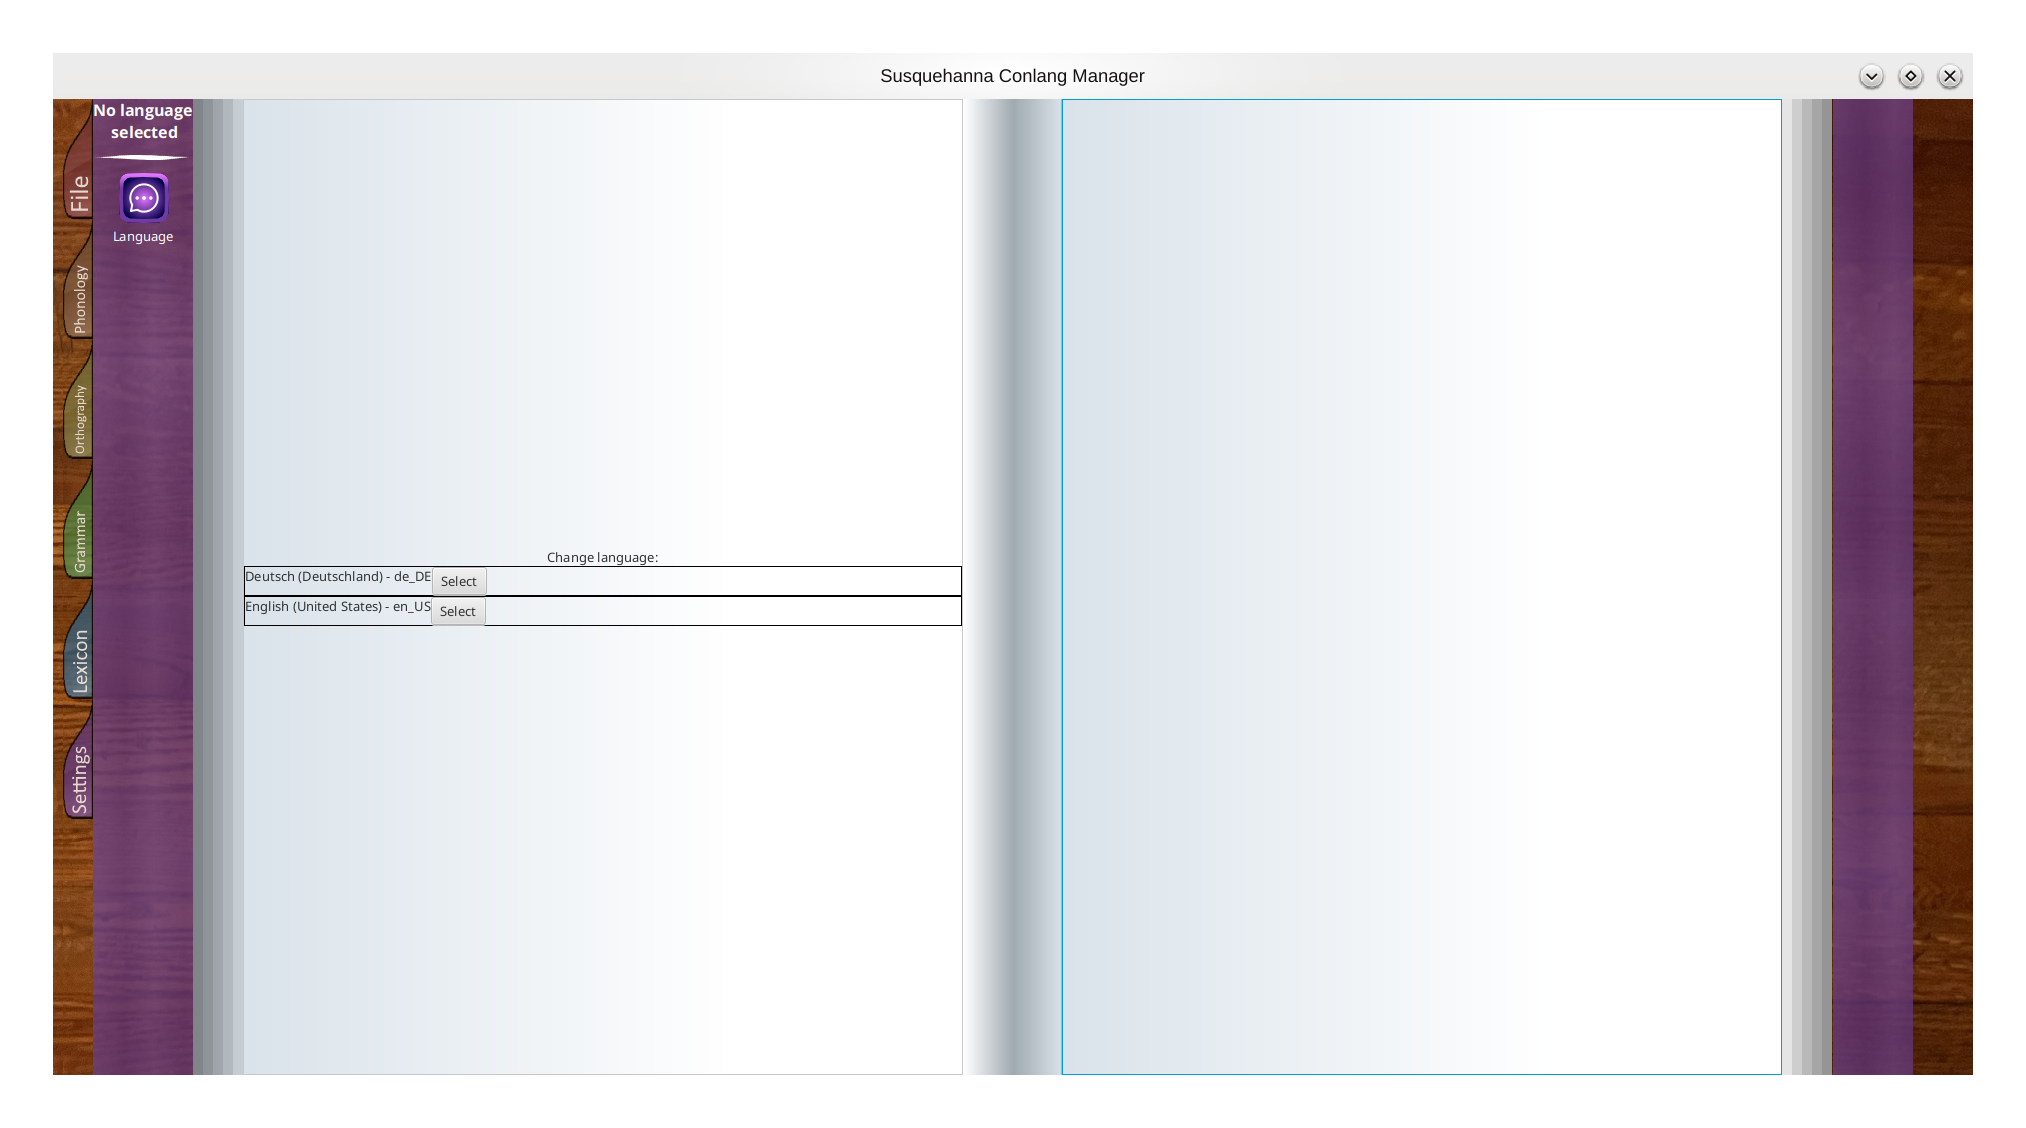
\includegraphics[width=1\linewidth]{img/settings-tab}
		\caption{The Settings tab, when first clicked.}
		\label{fig:settings-tab}
	\end{figure}
	The settings tab will be the place to change how Susquehanna works. Currently, the only setting that can be changed here is the language, however this is planned to be changed in the future.
	\newpage
	\section{Language}
	\begin{wrapfigure}{r}{0.4\textwidth}
		\centering
		
\includegraphics[width=0.2\textwidth]{img/language}
		\caption{The Language tool button.}
		\label{fig:language}
	\end{wrapfigure}
	The Language book allows one to change the language Susquehanna shows text in. Currently, there are two built-in languages, those being English (US) and German (Germany). These packs can be found in the Susquehanna directory under \mbox{\emph{localizationPacks}}. Localization packs added to this directory should automatically appear in the language selection menu. Each localization file is simply a list of text, so translating Susquehanna should be relatively simple. In the future, these files may contain things such as date formats, currency formats, and other things dependent on locale. Furthermore, the ability to create locale files for conlangs is planned for a future update.
	
	
	
\end{document}